% SW design
\clearpage

\section{Software design}

Herunder er de forskellige dele af softwaren kort beskrevet. 

\subsection{PC delen (JC)}

Softwaren til PC'en, er brugerens grænseflade til at kontrollere systemet. Her kan han manurære rundt i de forskellige menuer og udføre de forskellige ting som er beskrevet i UC beskrivelserne.

Nedenfor er der illustreret hvordan man kommer frem og tilbage i brugerinterfacet. Udover bruger input så kan CSS-hovedenheden give PC'en besked om at der ikke længere er logget ind hvilket vil sende brugeren fra main menu og tilbage til pre-login menuen. Der kan kun sendes babyalarm så længe brugeren står i main menuen og ikke har trykket på keyboardet endnu.

\begin{figure}[htbp] \centering
{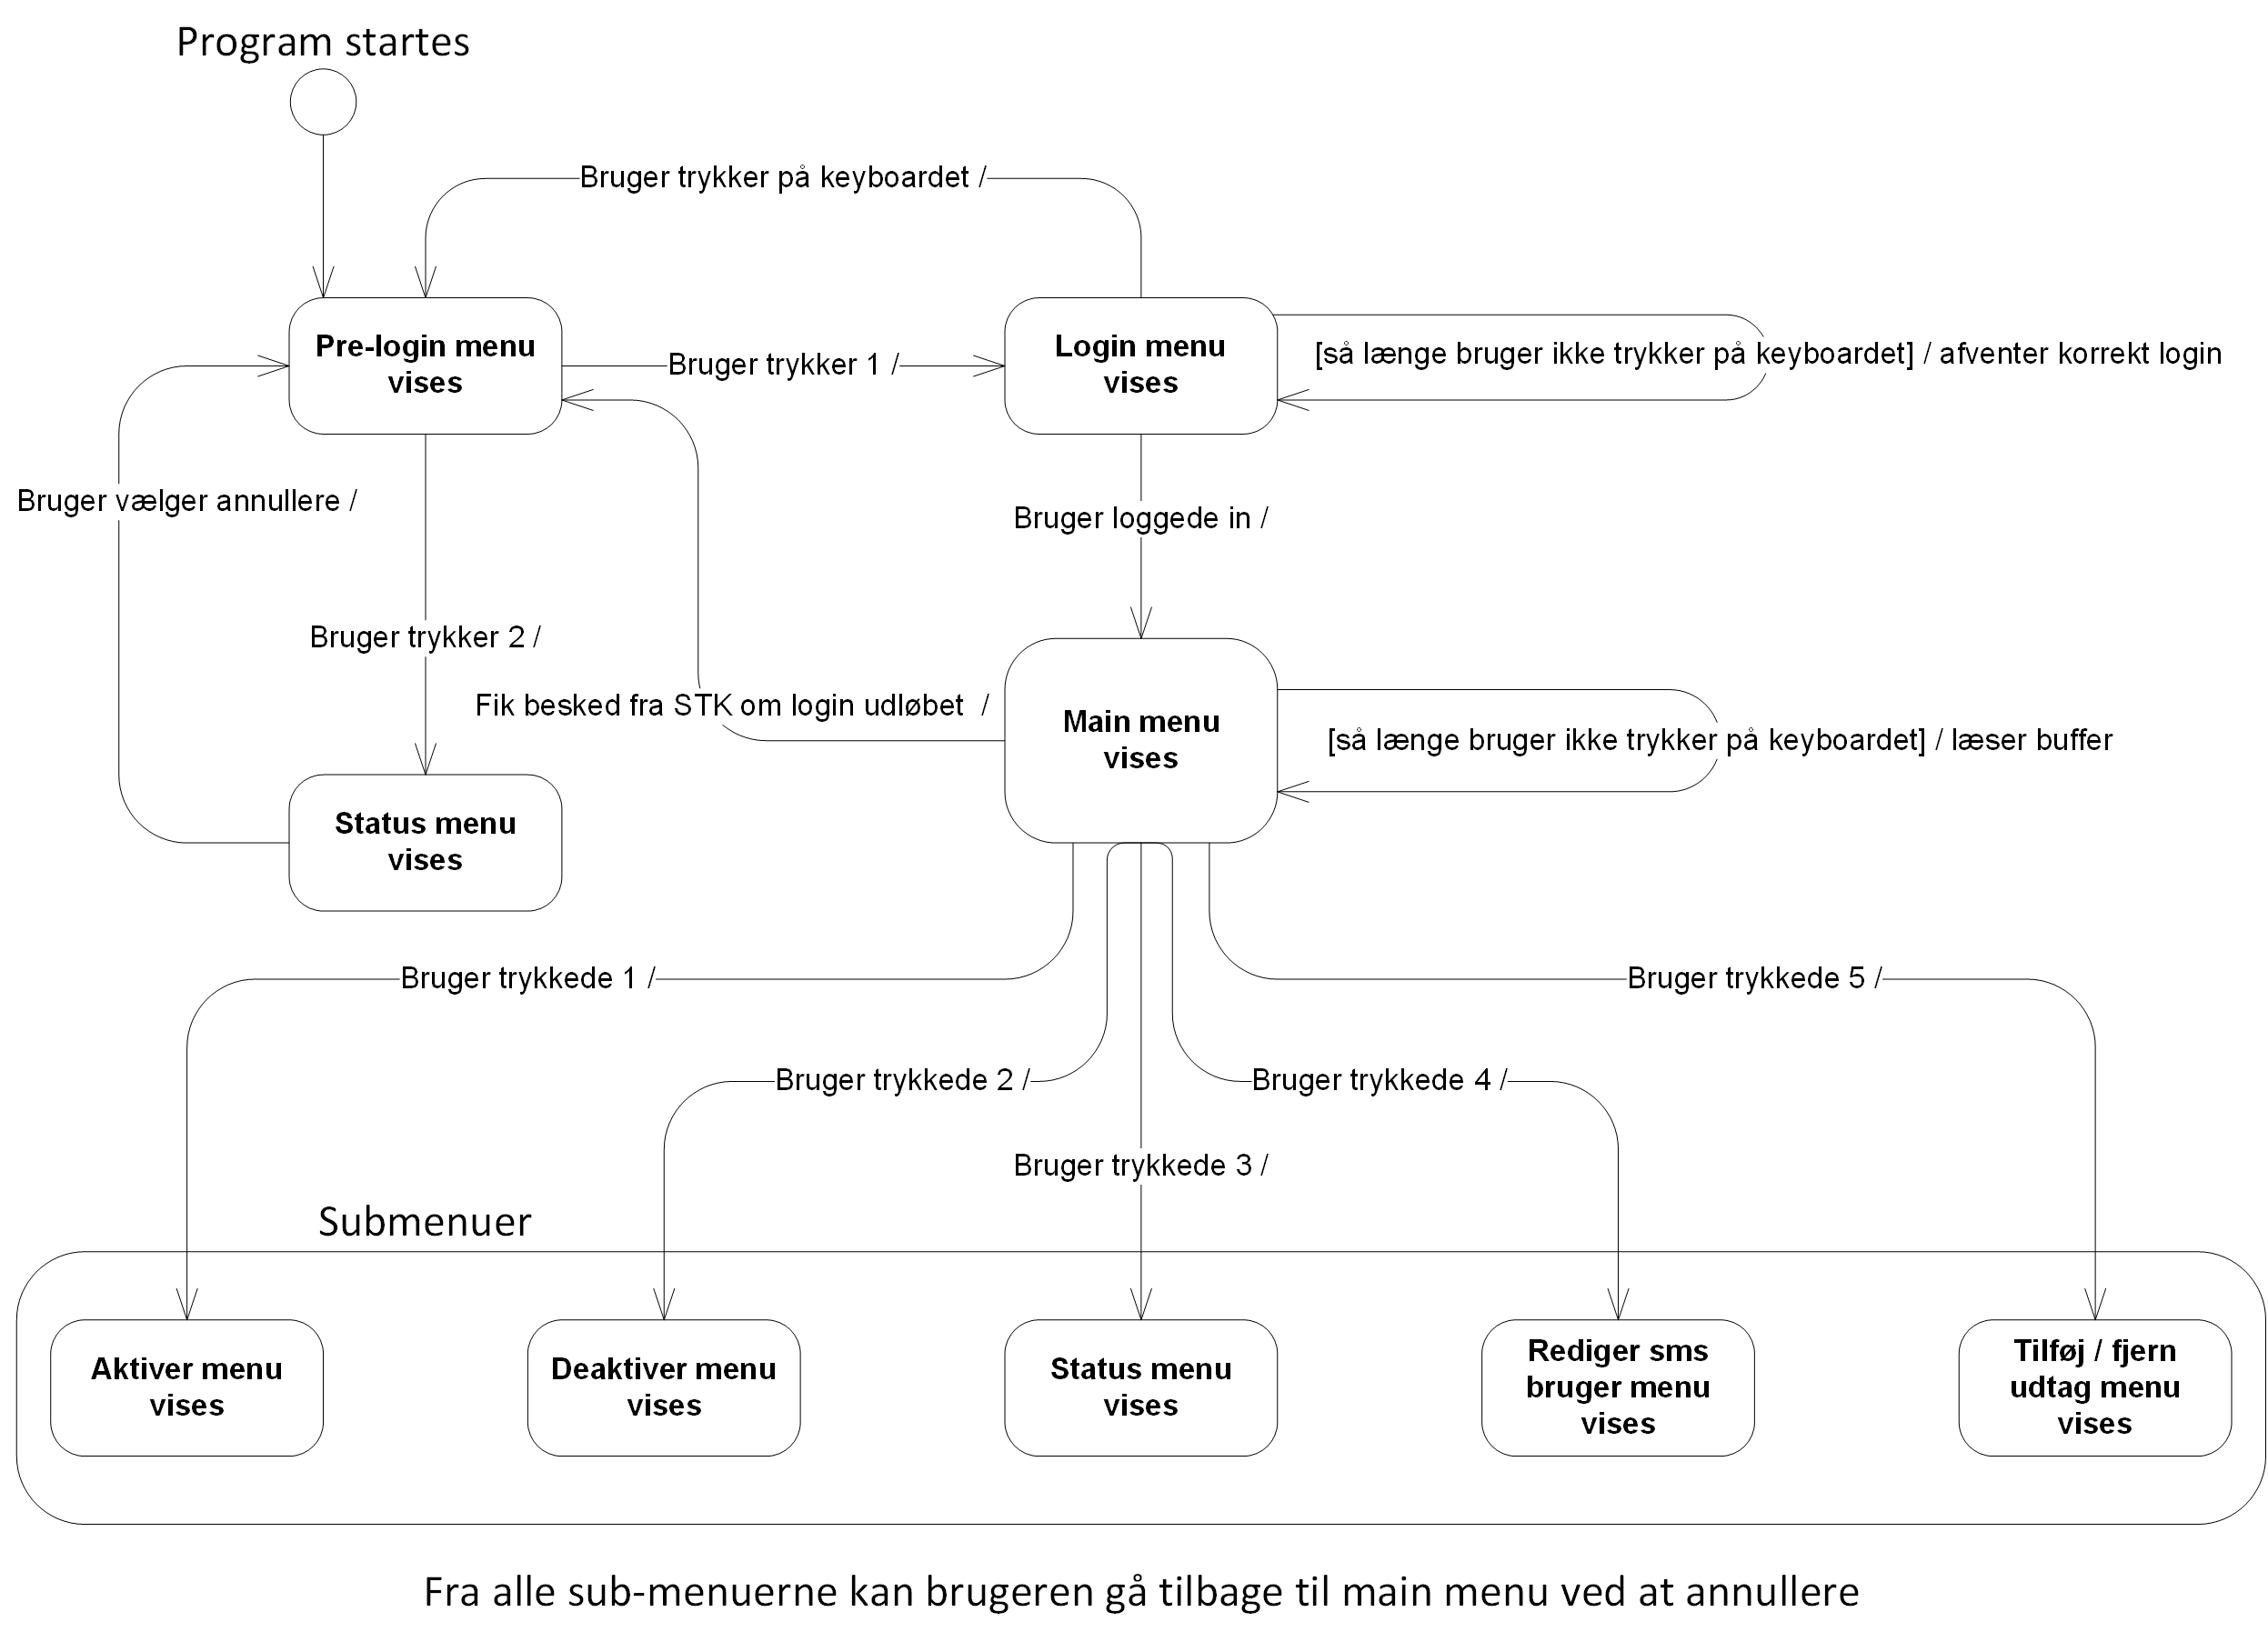
\includegraphics[width=\textwidth]{billeder/uml/state_machine_main}}
\caption{State machine diagram over brugerflade}
\label{fig:State machine diagram over brugerflade}
\end{figure}

En vigtig del af PC software er at vi kunne gemme alle de enheder brugeren har og hvilket telefonnummer brugeren har. Dette håndtere Hukommelse klassen som gemmer alt i en text fil og henter dataen ind under opstart. Således kan brugeren lukke programmet, åbne det igen og stadig have de samme enheder samt deres status og adresse. \ref{fig:Hukommelses header og udklip af text filen} Illustrere hvordan enhederne og telefonnummeret er gemt i text filen.

\begin{figure}[htbp] \centering
{\includegraphics[width=\textwidth]{billeder/uml/pc_dataview}}
\caption{Hukommelses header og udklip af text filen}
\label{fig:Hukommelses header og udklip af text filen}
\end{figure}

\subsection{X10-udtag delen (JSA)}

Objektorienteret programmeret software der styre X10-udtaget hvorfra der læses zero cross og signal input fra hardwaren og herefter udføre funktioner som beskrevet i use case beskrivelserne.

Når der læses et zero cross signal på interrupt INT1 benet køres en interrupt service rutinen som læser et højt- (logisk '1') eller lavt- (logisk '0') signal input på PD5 benet. Det modtaget bit bliver sendt til insertX10bit funktionen, som er vist i kodeudsnit figur \ref{fig:X10IF_insertX10bit}, som lager de modtaget bit løbende i et char array kaldet X10Array\_, funktion kontroller løbende de fire første pladser i arrayet for STX kommandoen, som er X10 signalets start kommando, når funktionen detekter at der er modtaget en STX kommando lager den de næste 24 bit der bliver modtaget i array\'et som derefter bliver sendt til funktionen unwrapX10Array. 

\begin{figure}[!htb]
\lstset{language=C++}
\begin{lstlisting}
void X10IF::insertX10bit(char X10bit)
{
	X10Array_[X10ArrayPlads_] = X10bit;
	
	if (X10ArrayPlads_ == 0 && X10Array_[0] != 1)
	{
		X10ArrayPlads_ = 0;
	}	
	else if (X10ArrayPlads_ == 1 && X10Array_[0] != 1 && X10Array_[1])
	{
		X10ArrayPlads_ = 0;
	}	
	else if (X10ArrayPlads_ == 2 && X10Array_[0] != 1 && X10Array_[1] != 1 && X10Array_[2])
	{
		X10ArrayPlads_ = 0;
	}
	else if (X10ArrayPlads_ == 3 && X10Array_[0] != 1 && X10Array_[1] != 1 && X10Array_[2] != 1 && X10Array_[3] != 0)
	{
		X10ArrayPlads_ = 0;
	}
	else if (X10ArrayPlads_ < 27)
	{
		X10ArrayPlads_++;
	}	
	else if (X10ArrayPlads_ >= 27)
	{
		unwrapX10Array(X10Array_);
		X10ArrayPlads_ = 0;
	}
}
\end{lstlisting}
\caption{Kodeudsnit for funktionen insertX10bit() fra X10IF.cpp}
\label{fig:X10IF_insertX10bit}
\end{figure}

I sekvens diagrammet, som vist i figur \ref{fig:X10_udtag_unwrapX10Array_SD}, er der vist hvordan unwrapX10Array funktionen dekoder det modtaget array. Metoden dekoder den modtaget X10 formateret kommando og adresse. Og sender herefter den dekodet adresse via den matchet dekodet kommando til den tilhørende controller.

\begin{figure}[!htb]
     {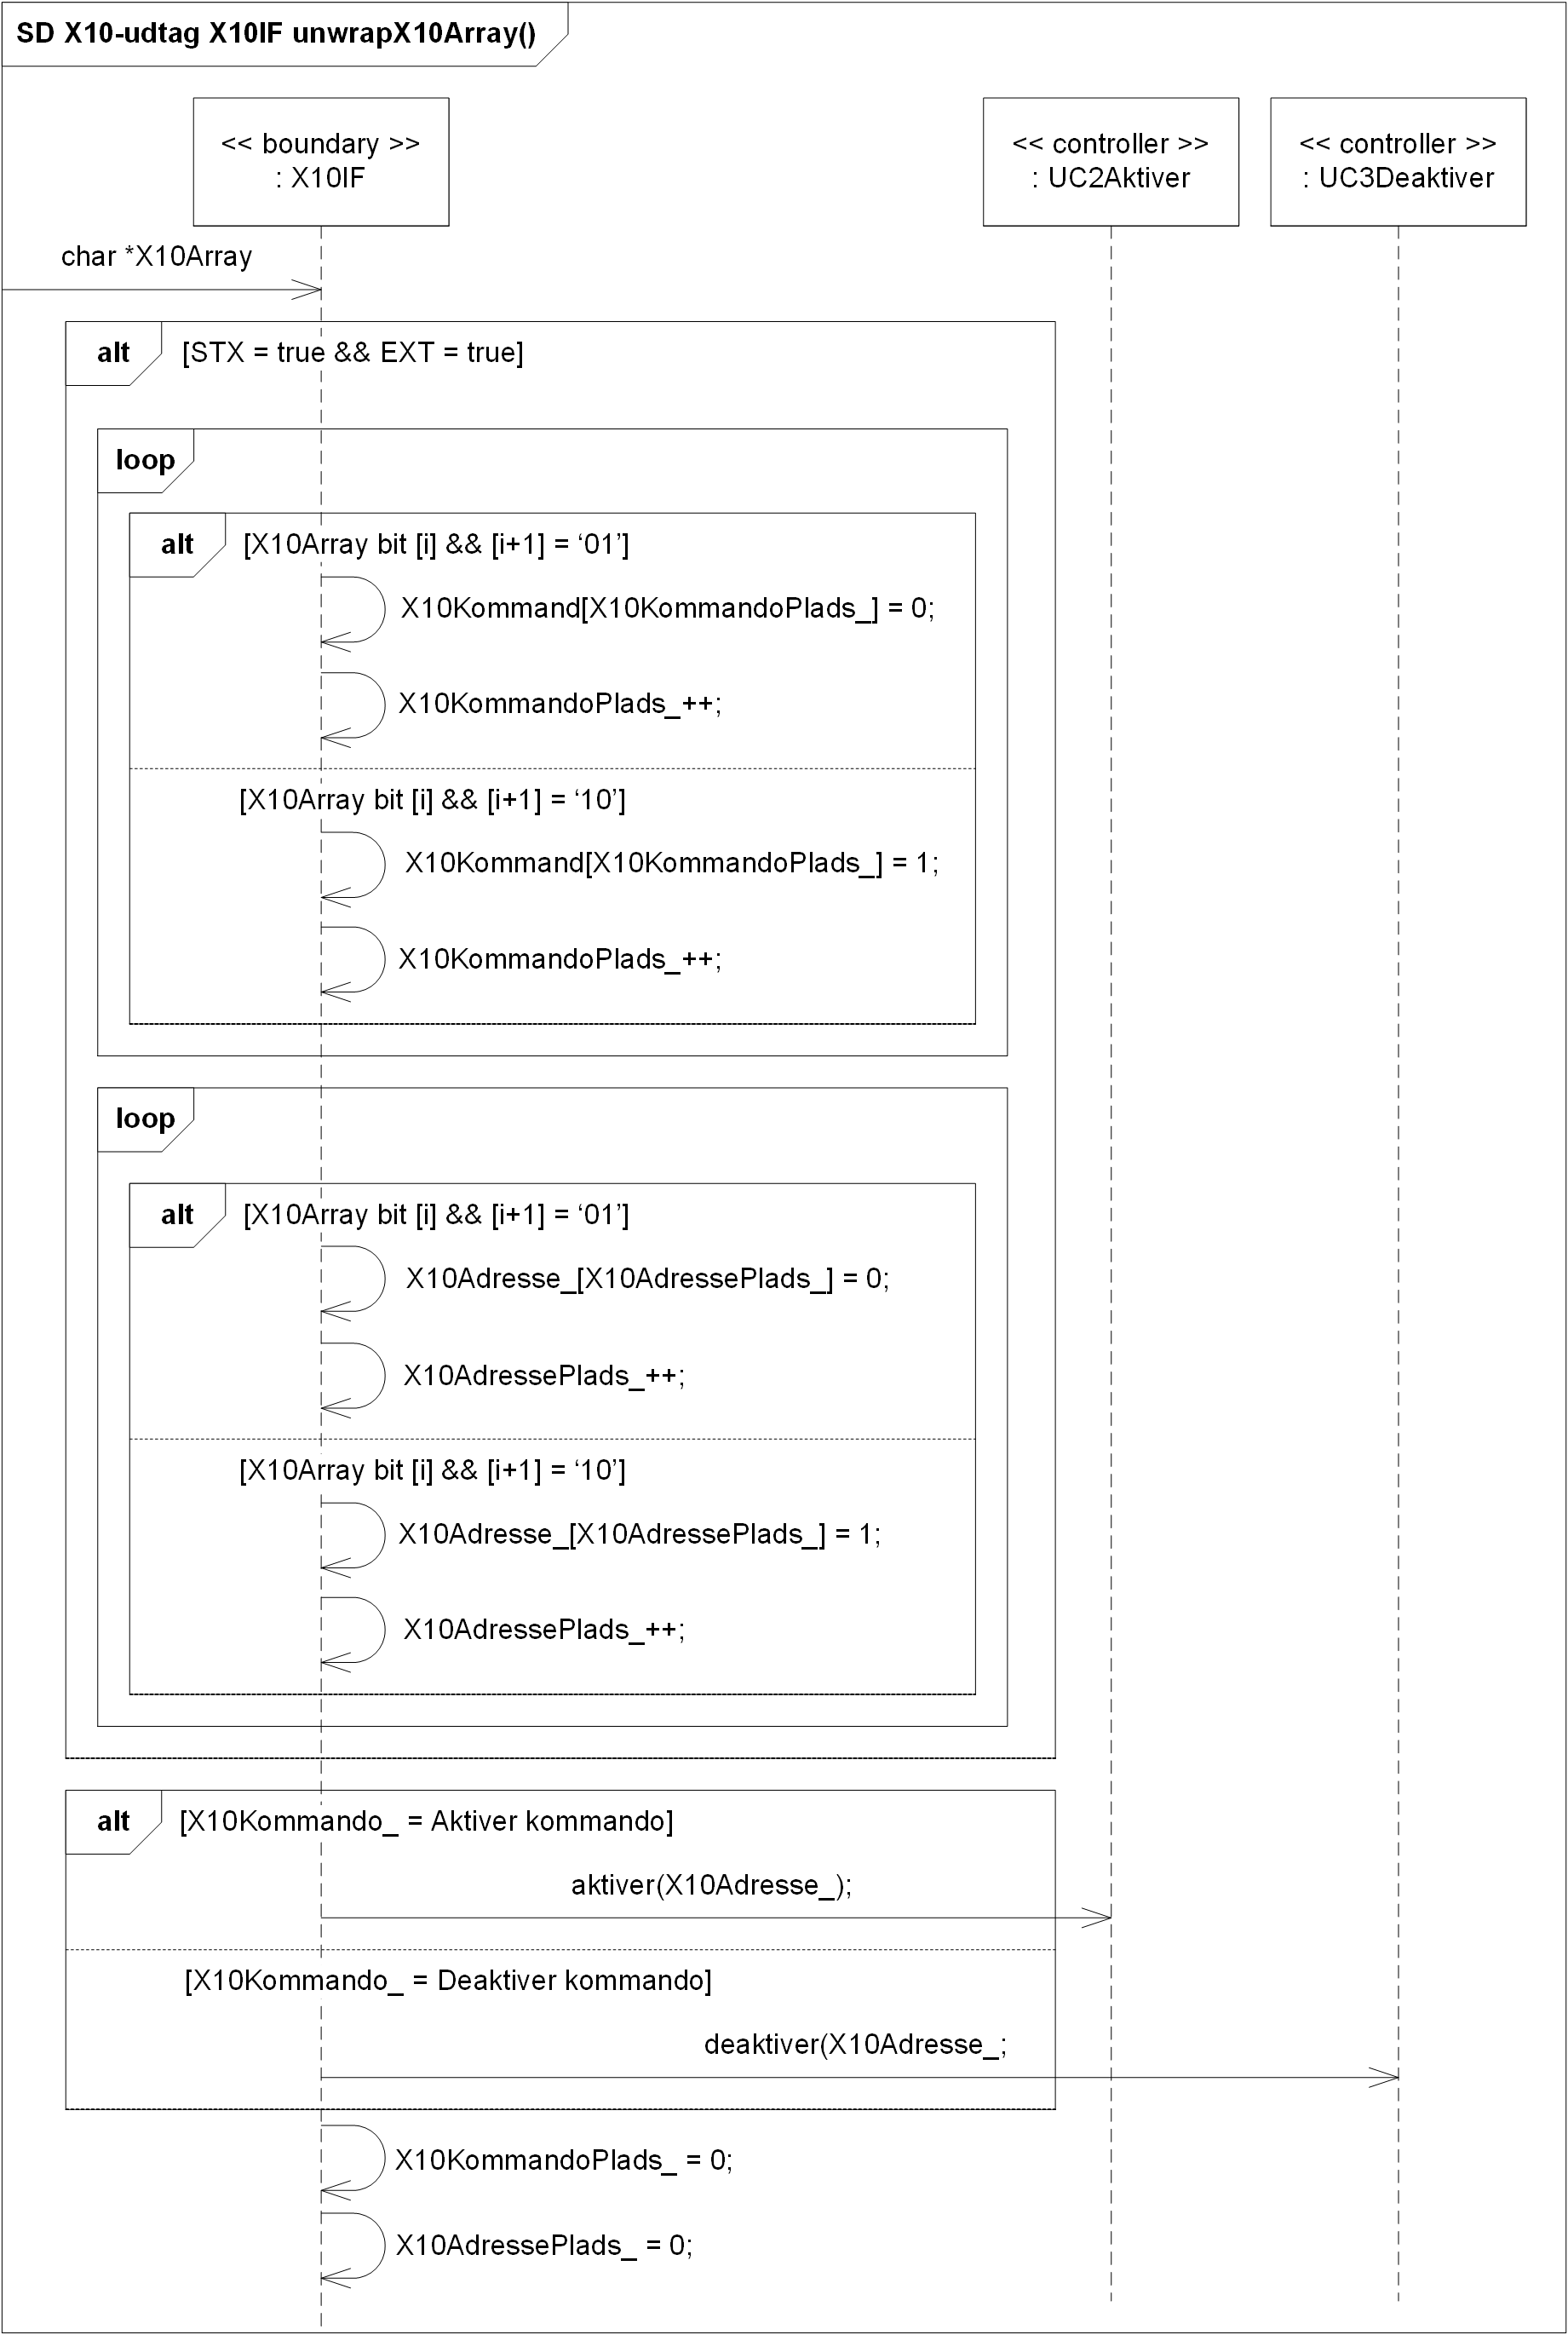
\includegraphics[width=\textwidth]{billeder/uml/X10-Udtag_unwrapX10Array_SD}}
     \caption{Sekvensdiagram for metoden unwrapX10Array() i X10IF klassen på X10-udtaget}
     \label{fig:X10_udtag_unwrapX10Array_SD}
\end{figure}

